\documentclass[../report.tex]{subfiles}

\begin{document}
	
\section{Introduction}

The goal of a Single Image Super Resolution Network is to take a low-resolution image and enhance its resolution by a factor of 2 or more. This is a regression task. The network takes an image in tensor form as input and outputs a larger tensor based on the scaling factor. The output tensor can be converted back into an image to visualize the upscaling result.\\
We can utilize a Convolutional Neural Network that employs several convolutional filters (learned during training) to leverage the regular structure of an image. A proposed architecture for this type of problem is shown in Figure \ref{fig:SR_architecture}.
\begin{figure}[tb]
	\caption{Super Resolution Architecture}
	\centering
	\label{fig:SR_architecture}
	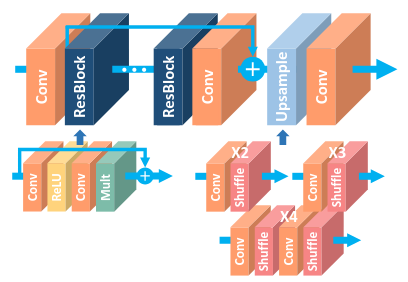
\includegraphics[scale=0.6]{../images/SISRN_Architecture.png}
\end{figure}
The network contains 3 main layers:
\begin{itemize}
	\item Convolutional
	\item Residual Block
	\item Upsample
\end{itemize}

\subsection{Convolutional And Residual Block Layers}

As shown in Figure \ref{fig:SR_architecture}, the first part of the network consists of an alternation between Convolutional and Residual blocks. The architecture of the Residual Blocks is illustrated in Figure \ref{fig:ResidualBlock_architecture}.
\begin{figure}[H]
	\caption{Residual Block Architecture}
	\centering
	\label{fig:ResidualBlock_architecture}
	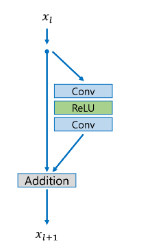
\includegraphics[scale=0.5]{../images/ResidualBlock.png}
\end{figure}
In the residual block layer, the input is processed through a convolutional filter, followed by a ReLU activation, another convolutional filter, and then summed with the original input for that layer before being passed to the next layer. The number of residual blocks in the network determines the depth of the network and is a parameter to be chosen during model selection.
The implementation of the Residual Block is shown in listing \ref{lst:ResidualBlock} .

\begin{lstlisting}[style=python,language=python, label={lst:ResidualBlock},caption={Residual Block implementation}]
from torch import nn


class ResidualBlock(nn.Module):

	def __init__(self, num_channels):
		super().__init__()
		self.conv1 = nn.Conv2d(num_channels, num_channels, kernel_size=3, padding=1)
		self.relu = nn.ReLU()
		self.conv2 = nn.Conv2d(num_channels, num_channels, kernel_size=3, padding=1)
	
	def forward(self, x):
		res = x
		out = self.conv1(x)
		out = self.relu(out)
		out = self.conv2(out)
		out += res
	return out
\end{lstlisting}

\subsection{Upsample and Output Layer}
The Upsample layer is the last layer responsible for increasing the dimensions of the tensor before passing it through the output convolutional layer. The implementation of the Upsample layer is shown in Listing \ref{lst:Upsample}. The component that actually performs the upscaling is the pixel shuffle operation.

\begin{lstlisting}[style=python, language=python, label={lst:Upsample}, caption={Upsample implementation}]
from torch import nn
	
class Upsample(nn.Module):
	
	def __init__(self, num_channel):
		super().__init__()
		self.conv = nn.Conv2d(num_channel, num_channel * 4, kernel_size=3, padding=1)
		self.shuffle = nn.PixelShuffle(2)
	
	def forward(self, x):
		out = self.conv(x)
		out = self.shuffle(out)
	return out
\end{lstlisting}

\end{document}


